% -*- mode: LaTeX; coding: utf-8 -*-
% Typeset with: XeLaTeX

\documentclass[a4paper,11pt]{article}
\usepackage{a4wide}

% Greek fonts
\RequirePackage[cm-default]{fontspec}
\defaultfontfeatures{Mapping=tex-text}
  % you may want to try: {FreeSerif} or {Times New Roman}
\setmainfont{Liberation Serif}
  % you may want to try: {FreeSans} or {Arial}
\setsansfont[Scale=MatchLowercase]{Liberation Sans}
  % you may want to try: {FreeMono} or {Courier New}
\setmonofont[Scale=MatchLowercase]{Liberation Mono}

% More packages and macros
\usepackage[inference]{semantic}
\usepackage{graphicx}
\graphicspath{ {./figures/} }
\usepackage{amsmath}
\usepackage[margin=2cm]{geometry}

\newcommand\nlambda[1]{\ensuremath{\lambda #1.\,}}
\newcommand\nred{\ensuremath{\longrightarrow}}

% Main document
\begin{document}
\title{Assignment 2}
\author{Thomas Pappas}
\maketitle

\section*{a}

Using the USCF Chimera software and after superimposing the the 6FAT and 1UWC proteins we get the following figures

\begin{figure}[h]
\centering
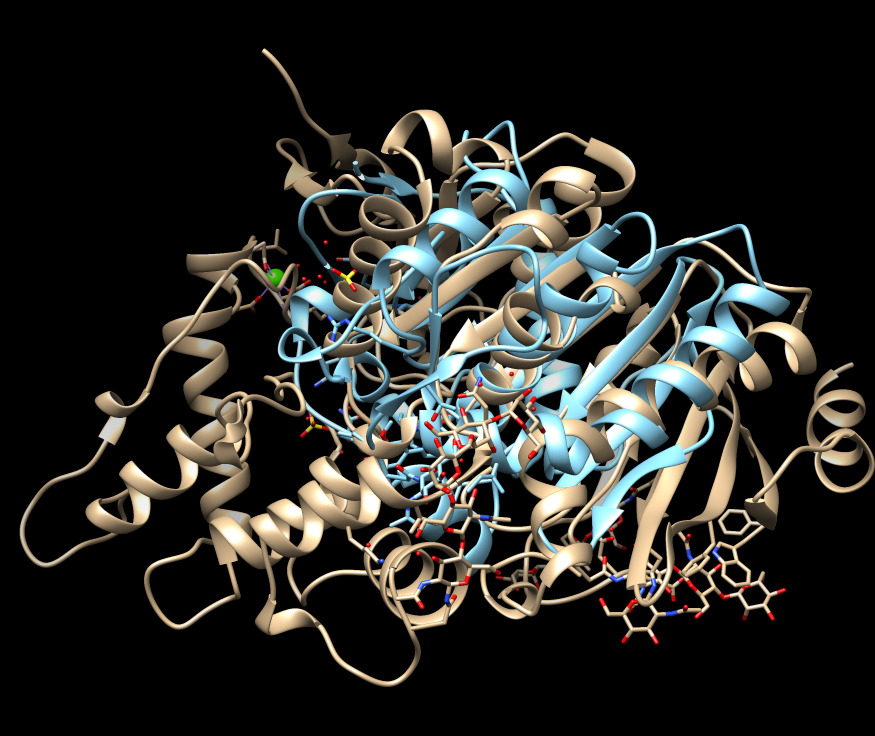
\includegraphics[width=0.4\textwidth]{superimposed}
\caption{The superimposed 3D structures}
\end{figure}
\begin{figure}[h]
\centering
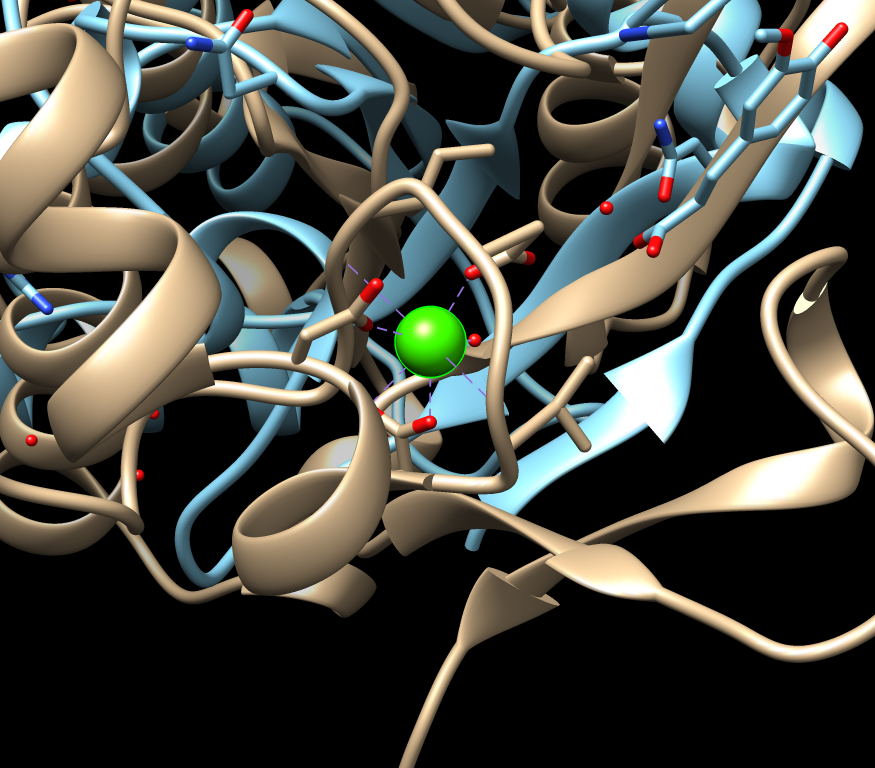
\includegraphics[width=0.4\textwidth]{superimposed_CA}
\caption{The superimposed 3D structures giving emphasis on the calcium binding site}
\end{figure}

% Reply log: RMSD between 20 pruned atom pairs is 1.037 angstroms; (across all 234 pairs: 22.983)
The c-RMSD as calculated by Chimera after superposition is
\begin{itemize}
  \item $1.037$ \AA \; between 20 pruned atom pairs
  \item $22.983$ \AA \; across all 234 pairs
\end{itemize}

%\section*{b}
%How to calculate the c-RMSD between two structures of different length? Homology? Alignment?

\section*{c}

We will take the coodinates for each residue's backbone atoms from the \verb|6FAT.pdb| file and we'll calculate the Caley-Menger (border) matrix $B$. We get:

\begin{small}
  \[B =\]
  \[\begin{pmatrix}
    0 & 1 & 1 & 1 & 1 & 1 & 1 & 1 & 1 & 1\\
    1 & 0 & 1.077665 & 3.000898 & 5.4746245 & 10.628379 & 15.5881445 & 16.357075 & 23.977149 & 31.7466575\\
    1 & 1.077665 & 0 & 1.173865 & 2.9497055 & 7.310758 & 10.1919535 & 10.845074 & 16.593745  & 24.1580125\\
    1 & 3.000898 & 1.173865 & 0 & 0.8908105 & 3.025239 & 5.0428305 & 5.417763 & 10.345519  & 15.9237015\\
    1 & 5.4746245 & 2.9497055 & 0.8908105 & 0 & 1.0730015 & 3.03894 & 4.8417535 & 9.9602605 & 15.778275\\
    1 & 10.628379 & 7.310758 & 3.025239 & 1.0730015 & 0 & 1.1697375 & 2.939012 & 7.337819 & 11.4252685\\
    1 & 15.5881445 & 10.1919535 & 5.0428305 & 3.03894 & 1.1697375 & 0 & 0.8883295 & 3.0552225 & 6.377039\\
    1 & 16.357075 & 10.845074 & 5.417763 & 4.8417535 & 2.939012 & 0.8883295 & 0 & 1.084853 & 3.1626245\\
    1 & 23.977149 & 16.593745 & 10.345519 & 9.9602605 & 7.337819 & 3.0552225 & 1.084853 & 0 & 1.1833645\\
    1 & 31.7466575 & 24.1580125 & 15.9237015 & 15.778275 & 11.4252685 & 6.377039 & 3.1626245 & 1.1833645 & 0
  \end{pmatrix}\]
\end{small}

\section*{d}

By running the Python code for $B$ \verb|numpy.linalg.matrix_rank(B)| we verify that $rank(B) = 5$.\\
Now in order to calculate the Gram matrix $G$, we will use the formula
\[
  G[i,j] := \frac{d_{i0}^2 - d_{ij}^2 + d_{j0}^2}{2}
\]
and while we can use the $B$ matrix to get $\frac{d_{ij}^2}{2}$, in order to calculate $d_{i0}$ and $d_{j0}$ we'll need to use the original coordinates. We therefore get:
\begin{footnotesize}
  \[G =\]
  \[
    \begin{pmatrix}
      5199.442025 & 5188.332704 & 5287.185963 & 5326.089175 & 5419.655414 & 5410.547521 & 5409.324072 & 5401.249837 & 5487.240252\\
      5188.332704 & 5179.378713 & 5278.98134 & 5318.582438 & 5412.941379 & 5405.912056 & 5404.804417 & 5398.601585 & 5484.797241\\
      5287.185963 & 5278.98134 & 5380.931697 & 5421.417825 & 5518.00339 & 5511.837671 & 5511.00822 & 5505.626303 & 5593.808044\\
      5326.089175 & 5318.582438 & 5421.417825 & 5463.685574 & 5561.332566 & 5555.2185 & 5552.961168 & 5547.3885 & 5635.330409\\
      5419.655414 & 5412.941379 & 5518.00339 & 5561.332566 & 5661.125561 & 5655.807696 & 5653.583903 & 5648.730935 & 5738.403409\\
      5410.547521 & 5405.912056 & 5511.837671 & 5555.2185 & 5655.807696 & 5652.829306 & 5651.486458 & 5648.865404 & 5739.303511\\
      5409.324072 & 5404.804417 & 5511.00822 & 5552.961168 & 5653.583903 & 5651.486458 & 5651.920269 & 5650.381255 & 5742.063407\\
      5401.249837 & 5398.601585 & 5505.626303 & 5547.3885 & 5648.730935 & 5648.865404 & 5650.381255 & 5651.011947 & 5743.588506\\
      5487.240252 & 5484.797241 & 5593.808044 & 5635.330409 & 5738.403409 & 5739.303511 & 5742.063407 & 5743.588506 & 5838.531794
    \end{pmatrix}
  \]
\end{footnotesize}

and by using SVD we get the new coordinates:
\begin{center}
  \[
    \begin{pmatrix}
      -0.720239668 & -3.29505773 & -1.06434145\\
      -0.719397583 & -1.95848694 & -0.462828815\\
      -0.733414994 & -1.34469699 & -0.384638014\\
      -0.739000952 & -1.33290190 & 0.827571807\\
      -0.752286576 & -0.772197814 & 1.08551735\\
      -0.751728771 & 0.755384109 & 1.13896831\\
      -0.751667006 & 1.37317774 & -0.0421124995\\
      -0.751193862 & 2.83776829 & -0.191918550\\
      -0.763282291 & 3.40972451 & -0.952375000
    \end{pmatrix}
  \]
\end{center}

thus achieving a c-RMSD with the initial coordinates (over all atoms) of $3.379948495065777 \times 10^{-13}$ \AA, which practically means the two structures are the same.

\vspace{5mm}

%\textit{Note: Intuitively it seems it would make more sense to calculate $G$ using only the values from $B$. However when taking $d_{i0} = 1$ the c-RMSD becomes $\sim 5$.}

\section*{e}

We implement the perturbation by increasing all values in $B$ by a percentage.
Then we recalculate $G$, run SVD to get the $U$ and $\Sigma$ values, take $S$ to be the $(3 \times 3)$ diagonal array with the three greatest values from $\Sigma$, and then check the c-RMSD between the original cooredinates and the points from $\sqrt{S}U^T$.

The algorithm tried 100 points between $1\%$ and $100\%$ (with a step of $1\%$) which was the incease applied to all values of $B$, and then run again for 10 more points in the space where the c-RMSD would go over $1$ to increase accuracy.

The conclusion was the max percentage of perturbation for c-RMSD to be less than $R = 1$ is around $88.61\%$.

\section*{f}

Here for calculating the c-RMSD we will take only the distances that are less than a number $T$.
For the rest of the points we will assume that the distance is $0$.
We will also keep $R = 1$ \AA.

\begin{center}
  \begin{tabular}{ ||c|c|| }
    \hline
    $T$ & c-RMSD\\
    \hline \hline
    30 & 4.848773458134514\\
    20 & 1.2941487875701954\\
    15 & 5.004258253300996\\
    10 & 5.243758773056963\\
    5 & 1.360263291246221\\
    4 & 1.3621607241108677\\
    3 & 1.3643224342718143\\
    2 & 1.15262288363306\\
    1 & 0.2292140768425968\\
    \hline
  \end{tabular}
\end{center}

And therefore for $T = 1$ we get the c-RMSD to be less than $R = 1$ \AA.

\end{document}
